\section{Numerical analysis}\label{sec:num}

We illustrate the models with a controlled toy instance generated by the functions in \texttt{src/models/cflp.py}. The goal is to show how adding sustainability levers alters siting and allocation choices; we do not attempt geographic calibration. Table~\ref{tab:instance} summarizes the instance: 10 candidate sites, 8 demand regions, total demand of 502.9 units, heterogeneous costs and capacities, and site-specific CO$_2$ and water factors. Latency eligibility is defined by a region-specific 60th-percentile distance threshold and a latency proxy weight $\phi=10$ in the objective.

\begin{table}[t]
  \centering
  \caption{Toy instance definition.}
  \label{tab:instance}
  \begin{tabular}{ll}
    \toprule
    Parameter & Value \\
    \midrule
    Number of candidate sites $|I|$ & 10 \\
    Number of regions $|R|$ & 8 \\
    Total demand & 502.9 \\
    Fixed cost range ($F_i$) & {[}248.9, 489.4{]} \\
    Operating cost range ($O_i$) & {[}56.3, 149.0{]} \\
    Capacity range ($C_i$) & {[}61.0, 84.2{]} \\
    CO$_2$ factor range ($e_i^{\mathrm{CO2}}$) & {[}0.23, 0.90{]} \\
    Water factor range ($w_i$) & {[}0.12, 0.53{]} \\
    Latency eligibility threshold & 60th percentile of distances per region \\
    Latency proxy weight ($\phi$) & 10.0 \\
    \bottomrule
  \end{tabular}
\end{table}
Table~\ref{tab:instance} shows heterogeneous costs, capacities, and impact factors with enough aggregate capacity to cover demand, ensuring multiple feasible siting patterns.

Three model variants are solved on this instance. The \emph{baseline} uses \eqref{eq:base-obj}--\eqref{eq:base-bounds} with latency proxy; sustainability is measured ex post. The \emph{capped-impact} model adds usage-based caps \eqref{eq:usage-caps} set at 85\% of the baseline CO$_2$ and water levels ($\Gamma_{\mathrm{CO_2}}=280.9$, $\Gamma_{\mathrm{W}}=106.2$). The \emph{scalarized} model replaces the objective with \eqref{eq:scalarized} and sweeps $(\lambda_{\mathrm{C}},\lambda_{\mathrm{W}})\in\{0,1,5,10,25,50\}^2$ to map cost–impact trade-offs.

\paragraph{Results.} Table~\ref{tab:kpi} reports portfolio KPIs. The baseline opens seven sites (S10,S2,S5,S6,S7,S8,S9) with total cost 3197.7, ex-post CO$_2$ 332.2, and water 139.4. Tightening caps pushes the model to replace S10 with a cleaner site (S4), cut CO$_2$ by 15\% and water by 24\%, at a 4.4\% cost increase; the opened set remains of size seven. Table~\ref{tab:siteshifts} details site-level flow shifts, with the largest reallocation from S10 to S4. The scalarized runs trace a smooth frontier: raising $(\lambda_{\mathrm{C}},\lambda_{\mathrm{W}})$ to (50,50) lowers CO$_2$ to 278.6 and water to 94.9 for a modest cost increase to 3311.9.

\begin{table}[t]
  \centering
  \caption{Baseline vs sustainability-aware KPIs.}
  \label{tab:kpi}
  \begin{tabular}{lllllll}
    \toprule
    Model Variant & Selected Sites & Total Cost & Total CO$_2$ & Total Water & Latency Proxy & Sites Opened \\
    \midrule
    Baseline & S10, S2, S5, S6, S7, S8, S9 & 3197.74 & 332.21 & 139.37 & 90.60 & 7 \\
    Capped-impact & S2, S4, S5, S6, S7, S8, S9 & 3337.18 & 280.91 & 106.19 & 115.53 & 7 \\
    Scalarized ($\lambda_{\mathrm{C}}{=}0$, $\lambda_{\mathrm{W}}{=}0$) & S10, S2, S5, S6, S7, S8, S9 & 3197.74 & 332.21 & 139.37 & N/A & N/A \\
    Scalarized ($\lambda_{\mathrm{C}}{=}50$, $\lambda_{\mathrm{W}}{=}50$) & S1, S2, S4, S5, S6, S8, S9 & 3311.86 & 278.60 & 94.91 & N/A & 7 \\
    \bottomrule
  \end{tabular}
\end{table}
Table~\ref{tab:kpi} highlights that modest cost increases (baseline to capped or scalarized) deliver meaningful CO$_2$/water reductions.

\begin{table}[t]
  \centering
  \caption{Site-level openings and flow shifts (baseline vs capped-impact).}
  \label{tab:siteshifts}
  \begin{tabular}{lrrlll}
    \toprule
    Site & Baseline ($x_i$) & Capped ($x_i$) & Baseline Flow & Capped Flow & Flow Change ($\Delta$) \\
    \midrule
    S1  & 0 & 0 & 0.00 & 0.00 & +0.00 \\
    S10 & 1 & 0 & 84.17 & 0.00 & $-84.17$ \\
    S2  & 1 & 1 & 62.25 & 62.25 & +0.00 \\
    S3  & 0 & 0 & 0.00 & 0.00 & +0.00 \\
    S4  & 0 & 1 & 0.00 & 69.47 & +69.47 \\
    S5  & 1 & 1 & 48.82 & 56.00 & +7.17 \\
    S6  & 1 & 1 & 73.50 & 81.02 & +7.52 \\
    S7  & 1 & 1 & 72.98 & 72.98 & +0.00 \\
    S8  & 1 & 1 & 81.92 & 81.92 & +0.00 \\
    S9  & 1 & 1 & 79.29 & 79.29 & +0.00 \\
    \bottomrule
  \end{tabular}
\end{table}
Table~\ref{tab:siteshifts} shows the main structural change: dropping S10 and adding S4, with flows reallocated accordingly.

Figure~\ref{fig:map} shows the baseline siting and flows. Figure~\ref{fig:selections} compares baseline vs capped siting choices side by side. Figures~\ref{fig:tradeoff_co2} and~\ref{fig:tradeoff_water} plot the scalarized cost--impact frontiers separately for CO$_2$ and water. Figure~\ref{fig:sensitivity} summarizes a cap-tightening sweep (100\% to 80\% of baseline impacts): as caps tighten, cost rises and the composition of opened sites adjusts, but feasibility is preserved down to 80\%.

\begin{figure}[t]
  \centering
  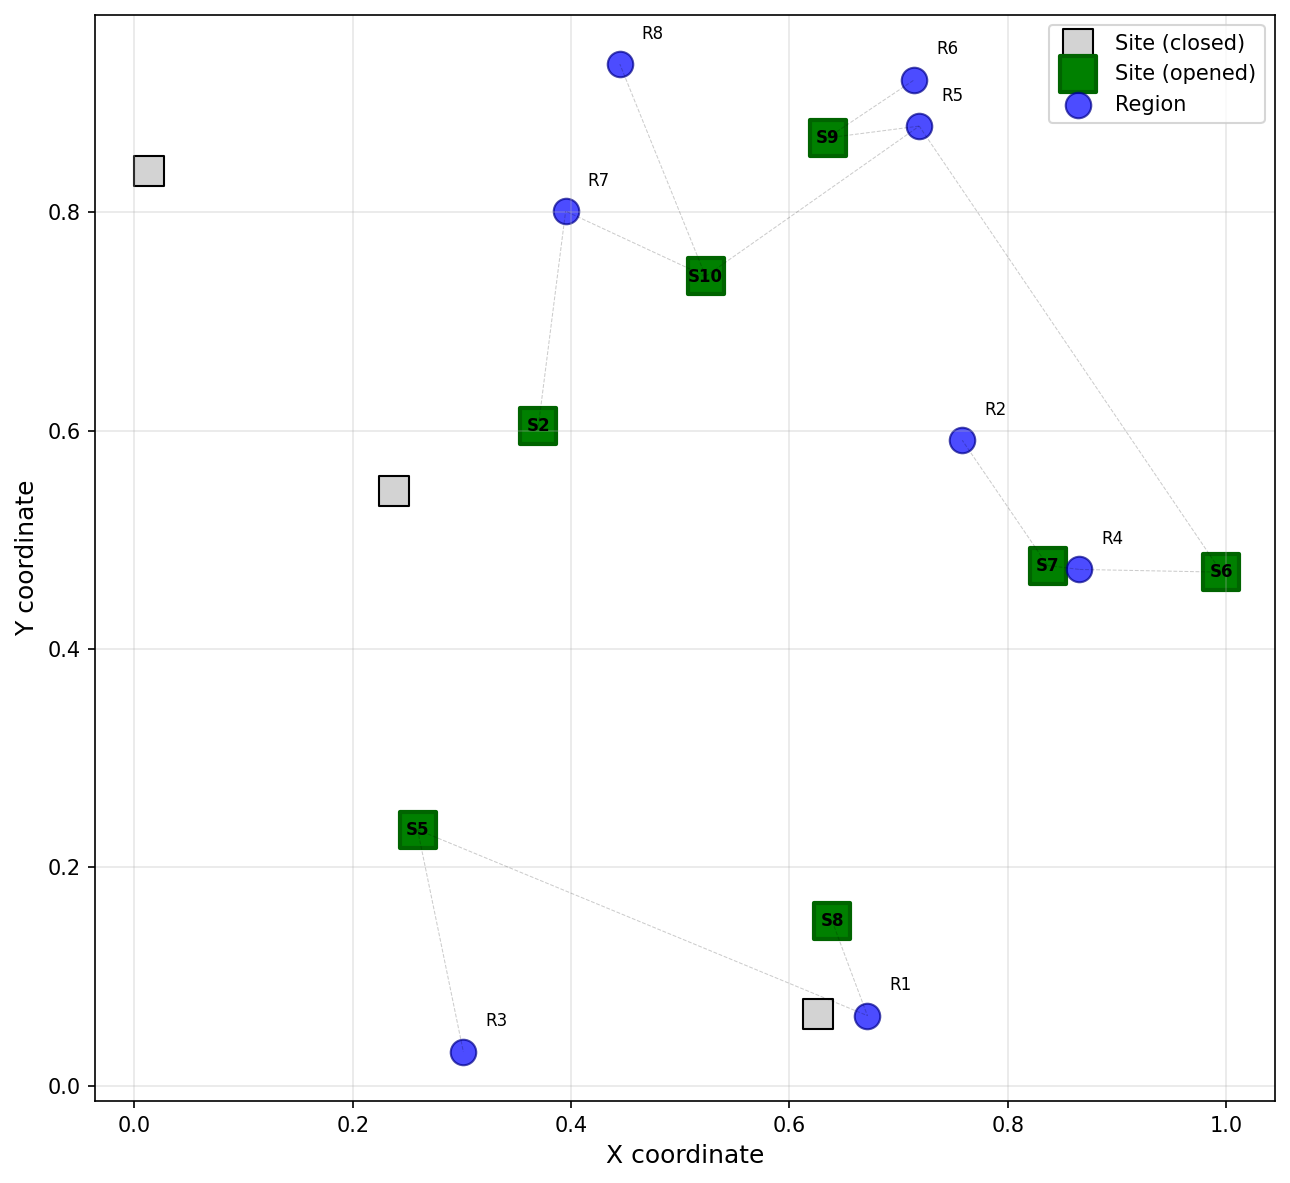
\includegraphics[width=0.7\textwidth]{fig/fig_map.png}
  \caption{Toy geography and baseline siting with flows.}
  \label{fig:map}
\end{figure}
Figure~\ref{fig:map} makes the baseline allocation pattern visible, including latency-driven eligibility constraints.

\begin{figure}[t]
  \centering
  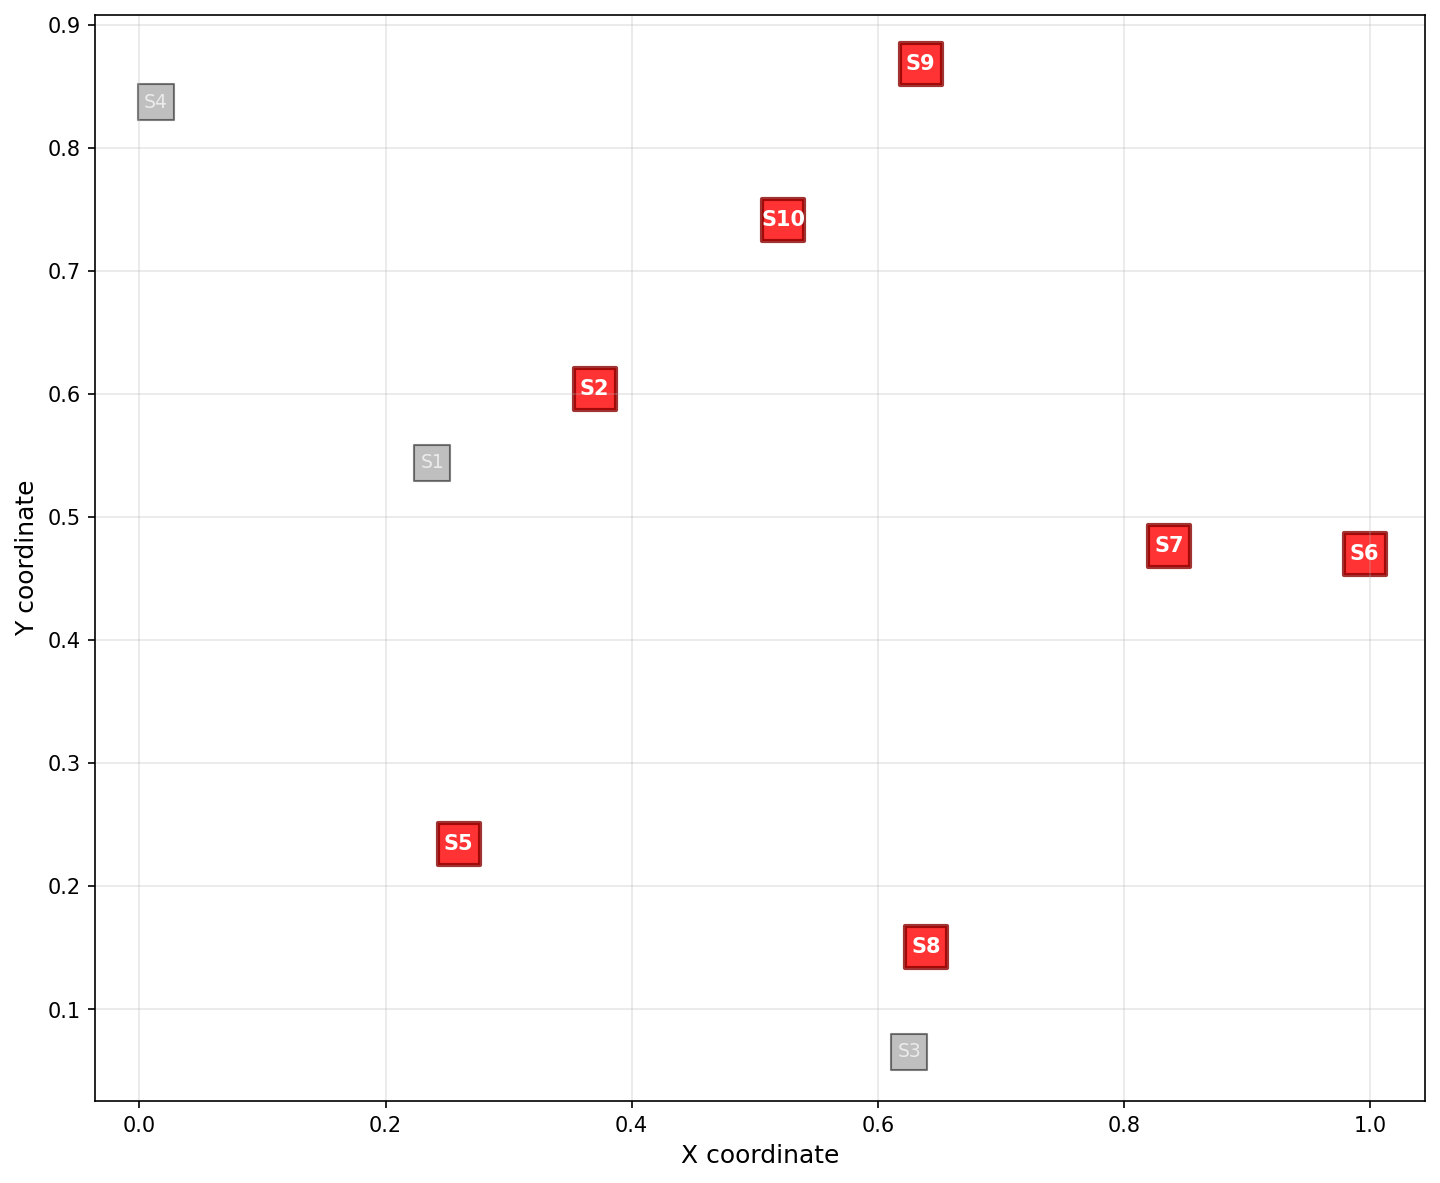
\includegraphics[width=0.48\textwidth]{fig/fig_baseline_selections.png}\hfill
  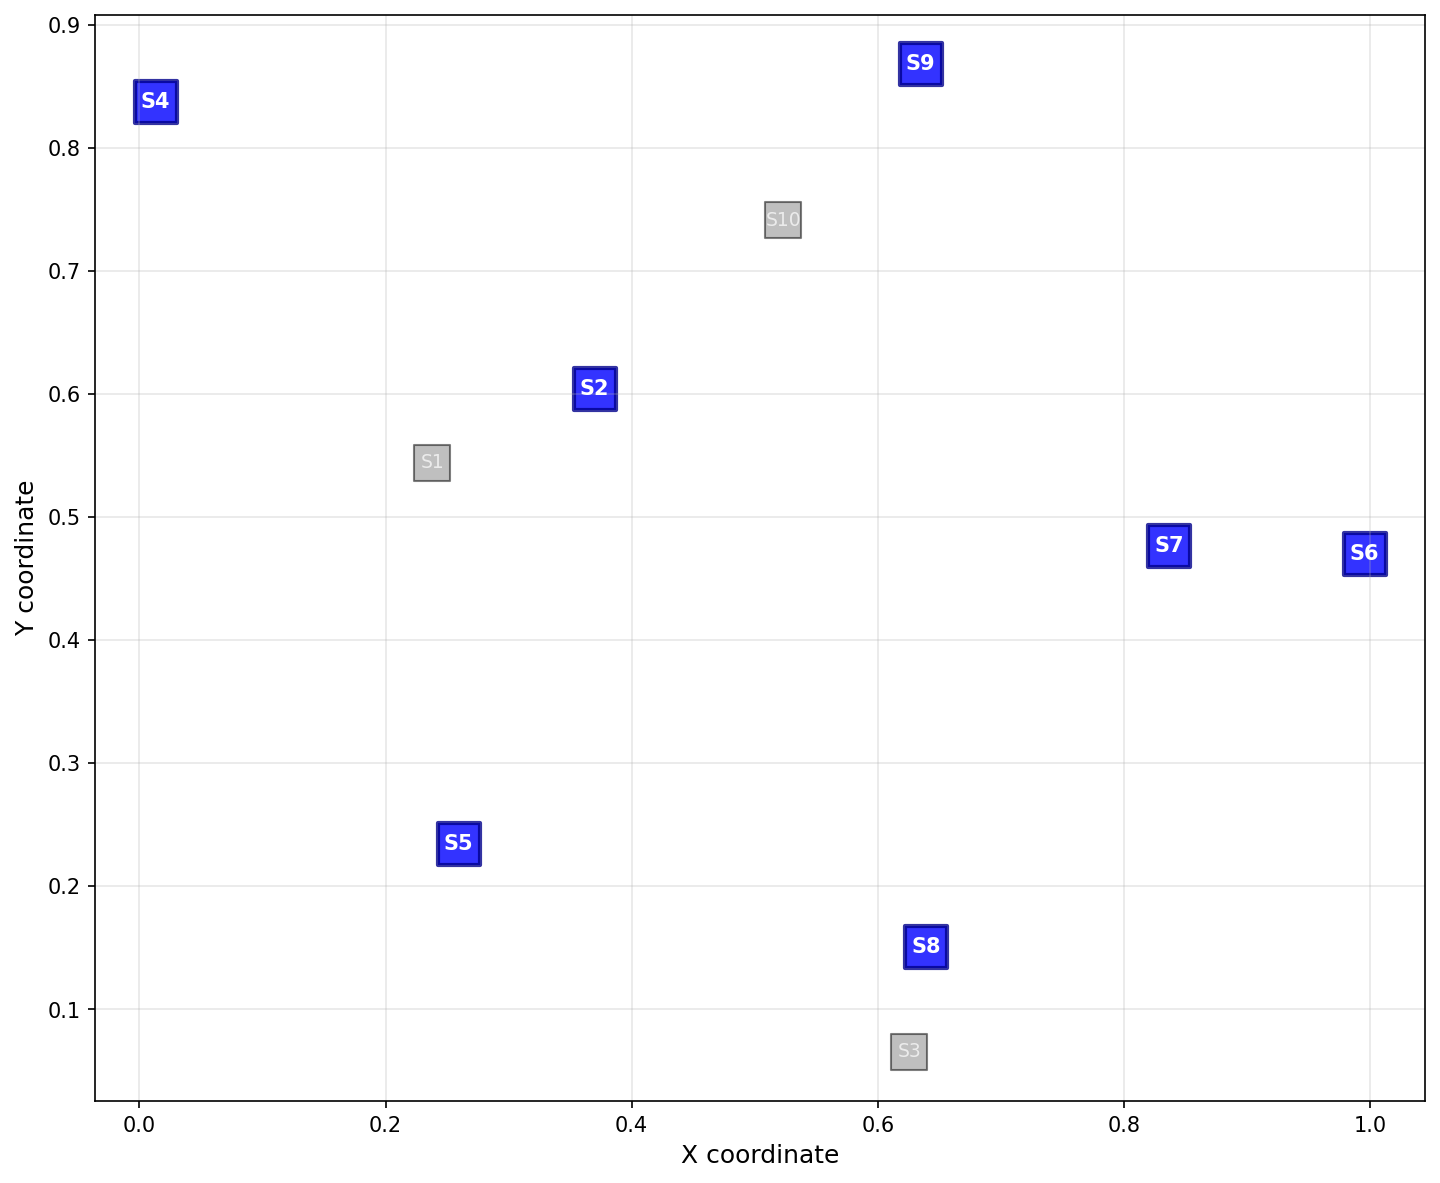
\includegraphics[width=0.48\textwidth]{fig/fig_capped_selections_85pct.png}
  \caption{Siting choices side by side: baseline (left) vs capped-impact (right).}
  \label{fig:selections}
\end{figure}
Figure~\ref{fig:selections} highlights the site substitution: S10 is replaced by S4 under the caps while maintaining seven openings.

\begin{figure}[t]
  \centering
  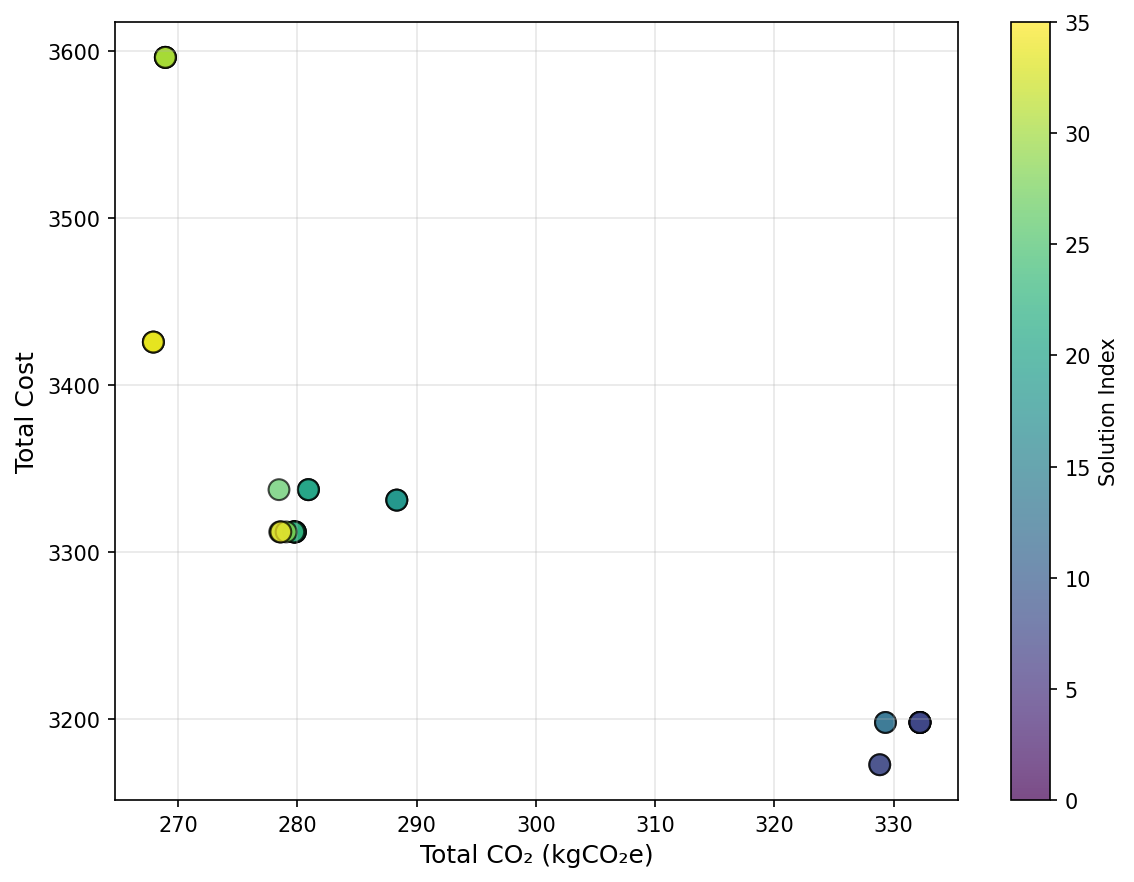
\includegraphics[width=0.7\textwidth]{fig/fig_tradeoff_cost_co2.png}
  \caption{Cost--CO$_2$ trade-offs from scalarized runs ($\lambda_{\mathrm{C}},\lambda_{\mathrm{W}}\in\{0,1,5,10,25,50\}$).}
  \label{fig:tradeoff_co2}
\end{figure}
Figure~\ref{fig:tradeoff_co2} shows the cost--CO$_2$ frontier: CO$_2$ can be cut from 332.2 to 267.9 (about $-19\%$) by paying roughly 7\% more cost (up to 3425).

\begin{figure}[t]
  \centering
  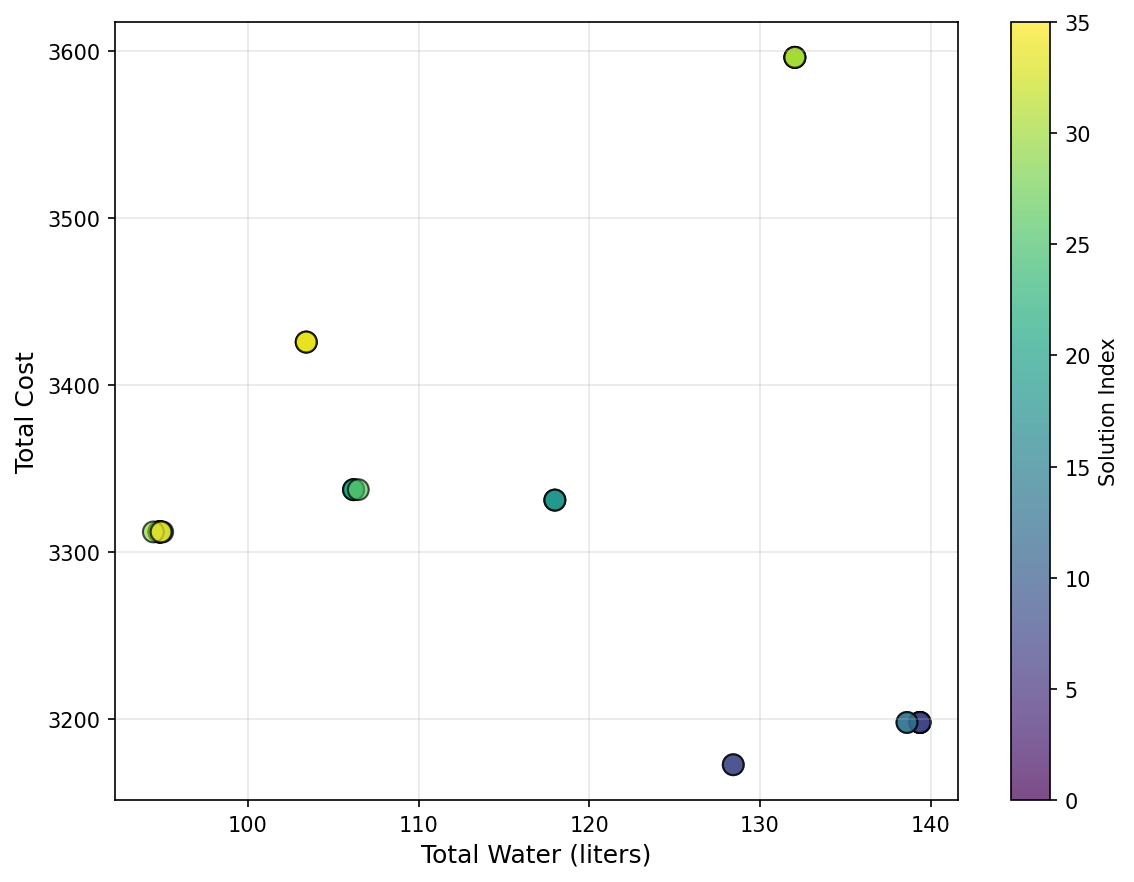
\includegraphics[width=0.7\textwidth]{fig/fig_tradeoff_cost_water.png}
  \caption{Cost--water trade-offs from scalarized runs ($\lambda_{\mathrm{C}},\lambda_{\mathrm{W}}\in\{0,1,5,10,25,50\}$).}
  \label{fig:tradeoff_water}
\end{figure}
Figure~\ref{fig:tradeoff_water} shows the cost--water frontier: water can be pushed down to 94.5 (about $-32\%$) with only a $\sim$3.6\% cost increase (cost $\approx$3312); heavier weights eventually raise cost without further water gains.

\begin{figure}[t]
  \centering
  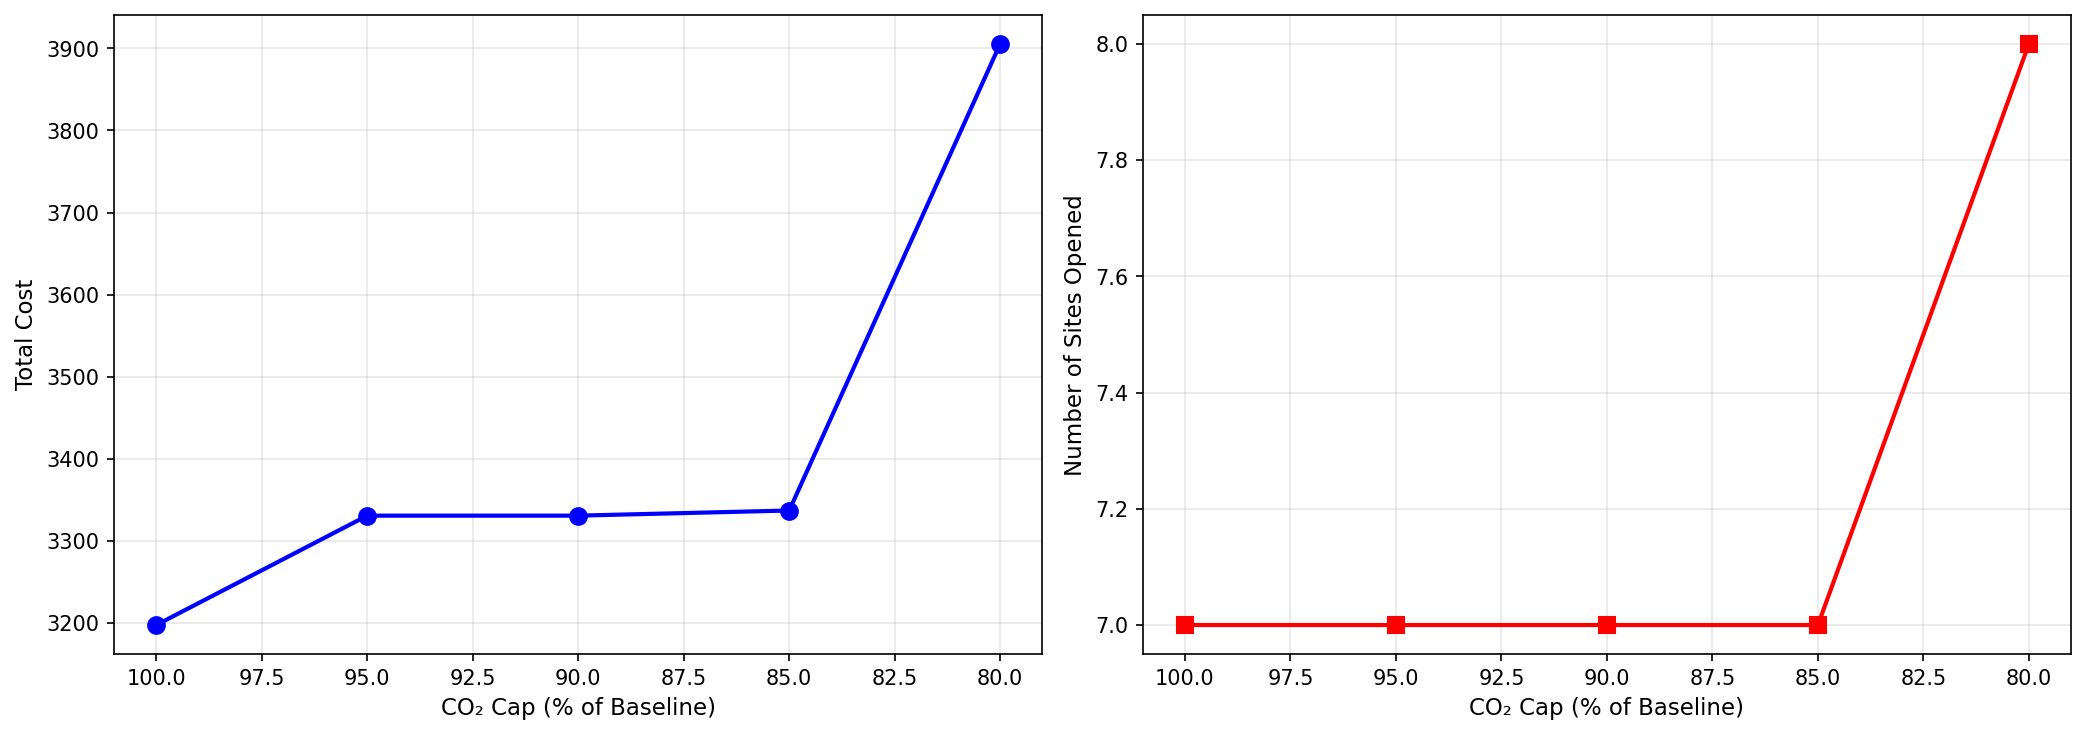
\includegraphics[width=0.7\textwidth]{fig/fig_sensitivity.png}
  \caption{Sensitivity to sustainability caps (percentage of baseline CO$_2$/water). Tightening caps raises cost and prompts site substitutions.}
  \label{fig:sensitivity}
\end{figure}
Figure~\ref{fig:sensitivity} shows monotone cost increases and opening-pattern shifts as caps tighten: from 100\% to 85\% impacts, cost rises mildly (3198$\to$3337) with seven openings; at 80\% the model needs eight openings and cost jumps to 3905, indicating a steeper trade-off near the feasibility boundary.

\paragraph{Reproducibility.} All experiments are scripted. Running \texttt{scripts/run\_all.py} reproduces the baseline, capped-impact, and scalarized runs and generates figures; \texttt{scripts/run\_sensitivity.py} tightens caps; \texttt{scripts/generate\_tables.py} exports Tables~\ref{tab:instance}--\ref{tab:siteshifts}. Generated assets live in \texttt{results/} and are copied to \texttt{latex/fig} for inclusion.
